\documentclass{article}
\usepackage[utf8]{inputenc}
\usepackage{graphicx, hyperref}
\graphicspath{ {./images/} }

\title{Specification of my Personal Computer}
\author{Richard Valo}
\date{\today}

\begin{document}

\maketitle

\section{Introduction}
\begin{itemize}
  \item PC Manufacturer         : LENOVO
  \item PC Model                : 30A6S0SE00
  \item Mather Board Model   : not accessible
  \item Max Number of RAMs   : 8 DIMM slots
  \item Max RAM              : 512GB (LRDIMM)/256GB (RDIMM)
  \item Number of Used Slots : 4
  \item Max Speed            : 2133 MHz
\end{itemize}
\href{https://www.getech.co.uk/pdf/p5001.pdf}{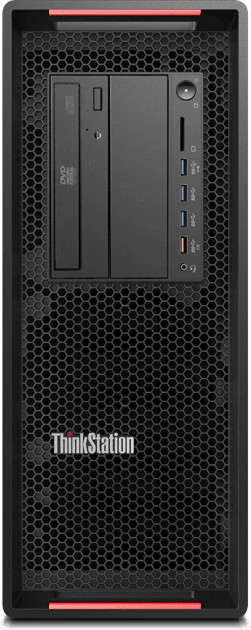
\includegraphics[height=8cm]{PC.jpg}}
\section{Random Access Memory}
Random-access memory (RAM) is a form of computer memory that can be read and changed in any order, typically used to store working data and machine code.A random-access memory device allows data items to be read or written in almost the same amount of time irrespective of the physical location of data inside the memory, in contrast with other direct-access data storage media (such as hard disks, CD-RWs, DVD-RWs and the older magnetic tapes and drum memory), where the time required to read and write data items varies significantly depending on their physical locations on the recording medium, due to mechanical limitations such as media rotation speeds and arm movement.
\begin{itemize}
  \item Model Number        : HMA451R7MFR8N-TF
  \item Memory form         : DIMM
  \item RAM type            : DDR4
  \item RAM Manufacturer        : Hynix Semiconductor 
  \item Speed               : 1600 MHz
\end{itemize}
\href{https://www.datasheets360.com/pdf/4058231500629532296}{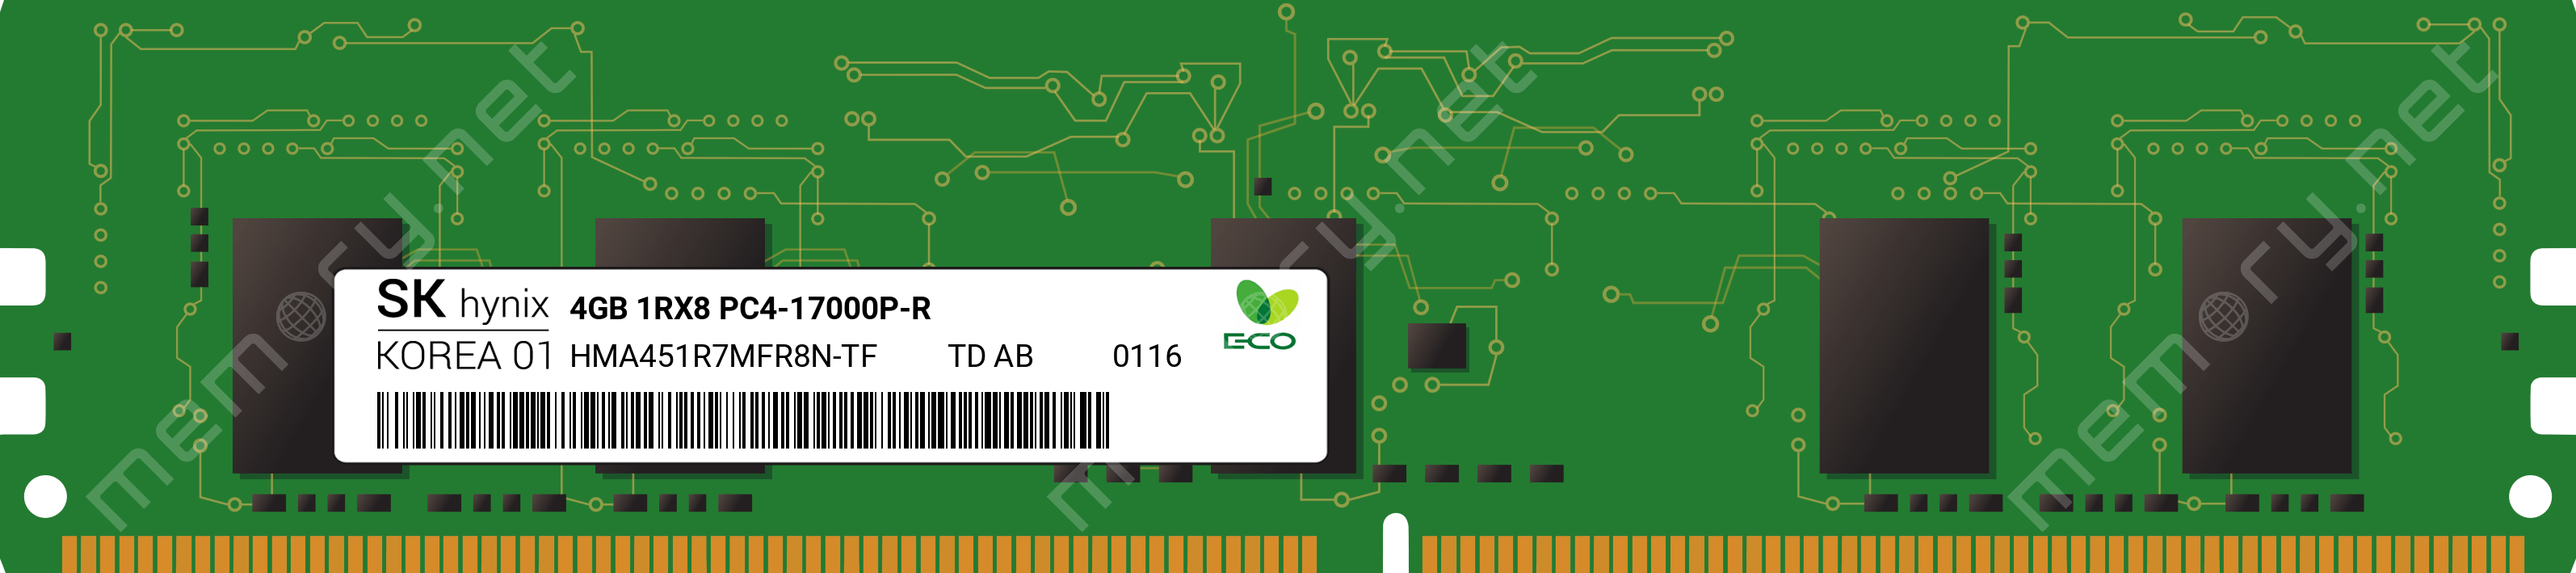
\includegraphics[width=\textwidth]{RAM.png}}
\section{Central Processing Unit}
A central processing unit (CPU), also called a central processor, main processor or just processor, is the electronic circuitry that executes instructions comprising a computer program. The CPU performs basic arithmetic, logic, controlling, and input/output (I/O) operations specified by the instructions in the program. This contrasts with external components such as main memory and I/O circuitry, and specialized processors such as graphics processing units (GPUs).
\begin{itemize}
  \item CPU Name                : Intel(R) Xeon(R) CPU E5-2609 v3 @ 1.90GHz
  \item Compatible RAM type        : DDR4 1600
  \item Max Memory Size            : 768 GB
\end{itemize}
\href{http://static6.arrow.com/aropdfconversion/bc27610082f0c9042063be09408c62b0895fa247/pgurl_5465333946064300.pdf}{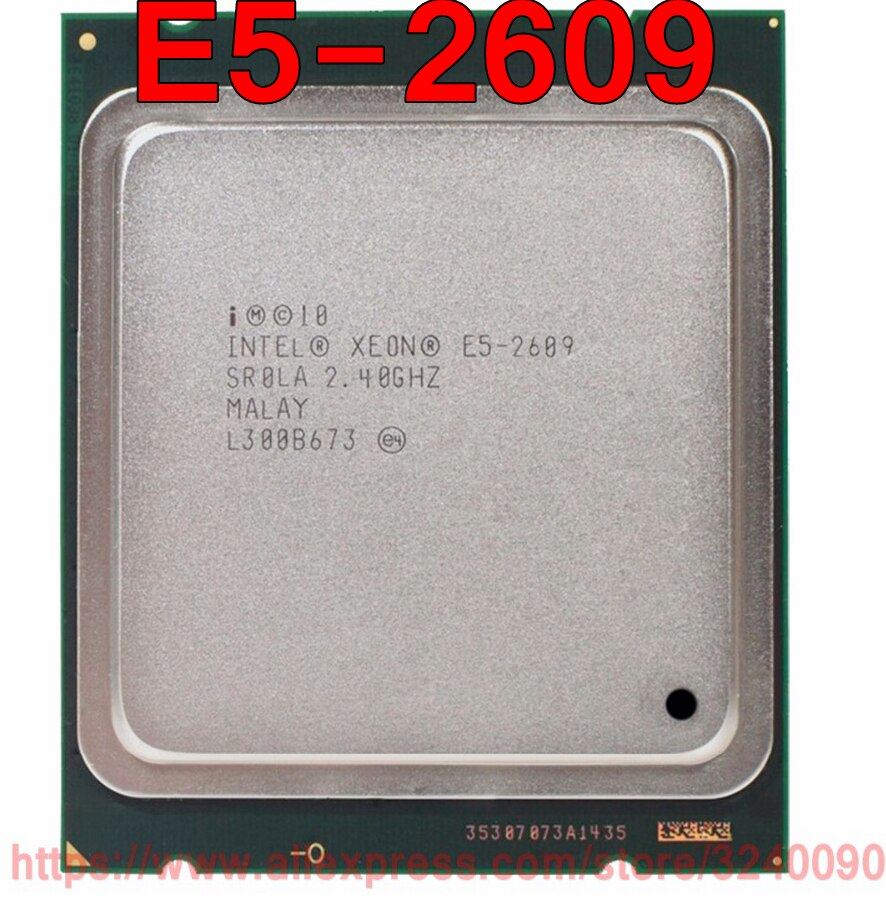
\includegraphics[height=4cm]{CPU.jpg}}
\section{Hard Disk}
A hard disk drive (HDD), hard disk, hard drive, or fixed disk is an electro-mechanical data storage device that stores and retrieves digital data using magnetic storage and one or more rigid rapidly rotating platters coated with magnetic material. The platters are paired with magnetic heads, usually arranged on a moving actuator arm, which read and write data to the platter surfaces. Data is accessed in a random-access manner, meaning that individual blocks of data can be stored and retrieved in any order. HDDs are a type of non-volatile storage, retaining stored data even when powered off. Modern HDDs are typically in the form of a small rectangular box.
\begin{itemize}
  \item Disk Type                : SSD 
  \item SSD Type            : MLC
  \item Disk Name                : ATA SanDisk SD6SB2M5
  \item Disk Capacity            : 476.94 GB
  \item Speed Read/Write    : 505/445MB/s
  \item Dimensions          : 2.5"
  \item Lifespan            : 80 TBW
  \item Disk Brand               : SanDisk
\end{itemize}


\href{https://www.mouser.com/datasheet/2/669/SanDisk_DataSheet_X210_08_06_13-805929.pdf}{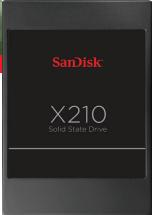
\includegraphics[height=8cm]{SSD.jpg}} 

\end{document}